\documentclass[12pt,a4paper]{article}
\usepackage[utf8]{inputenc}
\usepackage{amsmath}
\usepackage{amsfonts}
\usepackage{amssymb}
\usepackage{graphicx}
\title{A Comprehensive Study Of Face mask Detection}
\author{Rishab Kumar Vasista}
\begin{document}
\maketitle
\begin{abstract}
During these tough times , we need to implement every possible means to curb the spread the corona virus and Face mask detection is one of the most effective way to help the governing body enforce safety precautions i.e. wearing a mask properly with minimal amount of man power and equipment using existing infrastructure. This report goes through the various techniques used while detecting face masks and their advantages and disadvantages.
\end{abstract}
\section*{Introduction}
Image processing and computer vision go hand in hand for the development of models for Face-mask detection; This has become the need of the hour due to the covid-19 pandemic and this can be implemented in many ways. The virus spreads through droplets in the air and a face-mask is an important preventive measure that helps in curbing the coronavirus.
Face mask detection has been turned up to be an astonishing problem in the field of computer vision and image processing.Face detection has various use cases ranging from face recognition to capturing facial motions , where latter calls for the face to be revealed with very high precision. Due to the rapid advancement of the domain of machine learning algorithms , the jeopardies of face mask detection is yet to be well addressed. This technology is more relevant today because it used to detect faces not only static images and videos but also in real-time inspection and supervision . With the advancements of convolutional neural networks and deep learning algorithms , very high accuracy in image classification can be achieved .
\section*{Literature Review}
\section{The Viola Jones Algorithm}
The Viola Jones algorithm is the most popular algorithm used for facial detection. It is even used in the popular social media platforms like snapchat, instagram etc and in mobile phones for the face-unlock feature. In these platforms , it is mainly used to detect faces with Rapid object detection boosted with a cascade of simple features. This algorithm was invented by  Paul Viola and Michael Jones and it was published in 2001. Despite being an outdated framework, Viola-Jones is quite powerful and its application has proven to be exceptionally notable in real-time face detection.
Viola-Jones was designed for frontal faces, so it is able to detect frontal the best rather than faces looking sideways, upwards or downwards. Before detecting a face, the image is converted into grayscale, since it is easier to work with and there's lesser data to process. The Viola-Jones algorithm [1] first detects the face on the grayscale image and then finds the location on the colored image.
\\
\begin{figure}[hb!]
\centerline{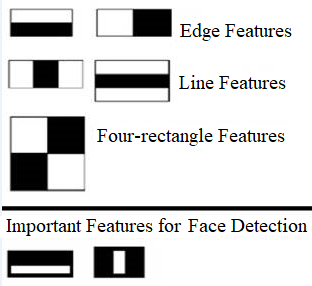
\includegraphics[scale=0.82]{haar_features.png}}
\caption{Haar features used in image processing}
\end{figure}
\\ \\
There are 3 types of Haar-like features that Viola and Jones identified in their research:
\begin{itemize}
\item Edge features
\item Line features
\item Four-sided features
\end{itemize}
These features help the machine understand what the image is. Imagine what the edge of a table would look like on a b\& w image. One side will be lighter than the other, creating that edge like b\& w feature as you can see in the picture above.
In the two important features for Face Detection, the horizontal and the vertical features describe what eyebrows and the nose, respectively, look like to the machine.\\
In the two important features for Face Detection, the horizontal and the vertical features describe what eyebrows and the nose, respectively, look like to the machine. While finding all the important features intensive calculations are performed . In order to reduce the amount of calculations, the concept of an integral image was introduced and this drastically reduced the computing time.Because Haar-like features are actually rectangular, and the integral image process allows us to find a feature within an image very easily as we already know the sum value of a particular square and to find the difference between two rectangles in the regular image, we just need to subtract two squares in the integral image. So even if you had a 1000 x 1000 pixels in your grid, the integral image method makes the calculations much less intensive and can save a lot of time for any facial detection model.
\subsection{Haar Features}
Haar like features are named after Alfred Haar, a Hungarian mathematician in the 19th century who developed the concept of Haar wavelets (kind of like the ancestor of haar like features)[2]. The features below show a box with a light side and a dark side, which is how the machine determines what the feature is. Sometimes one side will be lighter than the other, as in an edge of an eyebrow. Sometimes the middle portion may be shinier than the surrounding boxes, which can be interpreted as a nose.
\\
\begin{figure}[h!]
\centerline{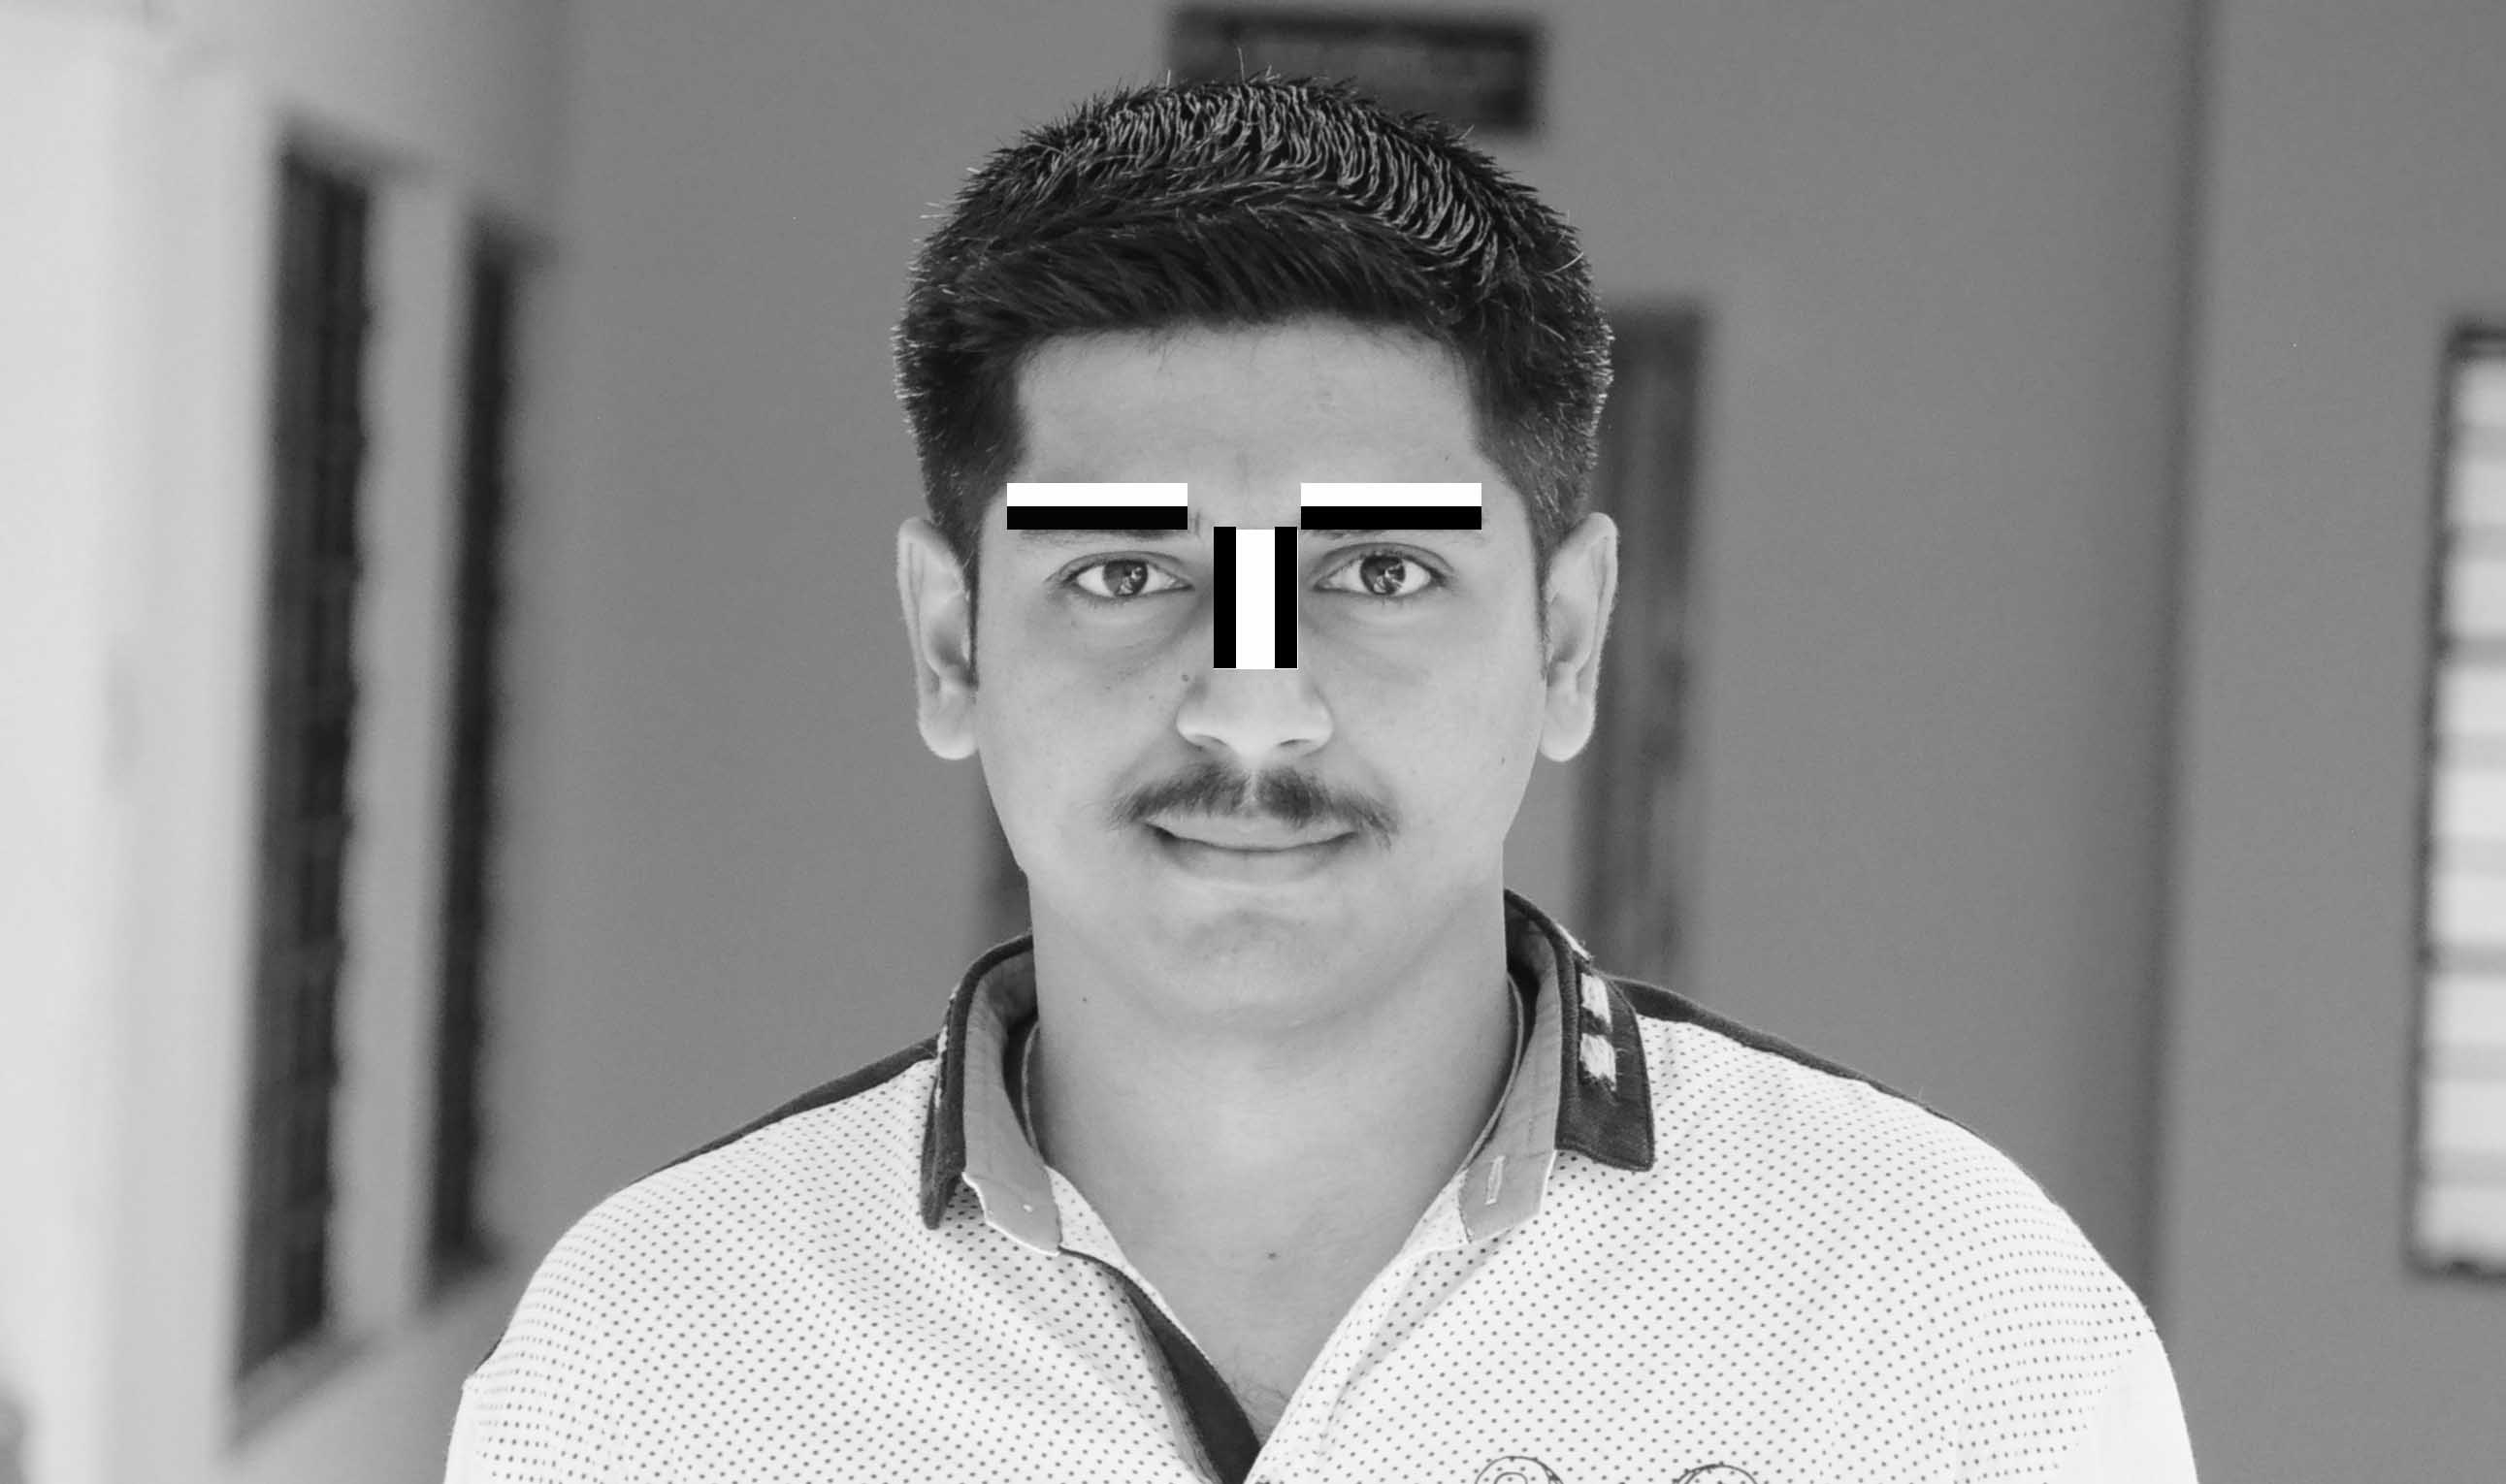
\includegraphics[scale=0.5]{haar_nose.jpg}}
\caption{Haar features for the nose and eyebrows}
\label{fig 2}
\end{figure}
\\
\subsection{Integral image}
An Integral image is where each pixel represents the cumulative sum of a corresponding input pixel with all pixels above and left of the input pixel. This algorithm enables rapid calculation of summations over image sub-regions. Any rectangular subset of such sub-region can be evaluated in constant time.[1]
This concept was introduced by Viola \& Jones and is also known as Summed Area Table.This allows fast computation of rectangular image features since they enable the summation of image values over any rectangle image region in constant time.The integral image at location (x,y) contains
the sum of the pixels above and to the left of x,y inclusive:\[ii(x,y)=\sum_{x'\leqslant x,y'\leqslant y} i(x',y') \] \\
\begin{figure}[ht!]
\centerline{\includegraphics[scale=0.7]{integral_image.png}}
\caption{The sum of the pixels within the rectangle D can be computed with four array references. The value of the integral image at location 1 is the sum of pixels in the rectangle A. The value at location 2 is A+B, at location 3 is A+C, and at location 4 is A+B+C+D. The sum within D can be calculated as 4+1-(2+3). }
\label{fig 3}
\end{figure}
where ii(x,y) is the integral image and i(x,y) is the original image. Using the following pair of recurrences:\[ s(x,y) = s(x,y-1)+i(x,y) .....(1) \] \[ii(x,y) = ii(x-1,y)+s(x,y) .....(2) \] \\
(where s(x,y) is the cumulative row sum, s(x,-1)=0 , and ii(-1,y)=0) the integral image can be computed in one pass over the original image.
Using the integral image any rectangular sum can be computed in four array references (see Figure 3). Clearly the difference between two rectangular sums can be computed in eight references. Since the two-rectangle features defined above involve adjacent rectangular sums they can be computed in six array references, eight in the case of the three-rectangle features, and nine for four-rectangle features.
\subsection{AdaBoost Algorithm}
AdaBoost algorithm, short for Adaptive Boosting, is a Boosting technique that is used as an Ensemble Method in Machine Learning. It is called Adaptive Boosting as the weights are re-assigned to each instance, with higher weights to incorrectly classified instances. Boosting is used to reduce bias as well as the variance for supervised learning. It works on the principle where learners are grown sequentially. Except for the first, each subsequent learner is grown from previously grown learners. In simple words, weak learners are converted into strong ones. Adaboost algorithm also works on the same principle as boosting, but there is a slight difference in working.
The Viola-Jones method uses a variant of AdaBoost learning where the algorithm is used both to select a small set of features and train the classifier. In its original form,the AdaBoost learning algorithm is used to boost the classification performance of a simple (sometimes called weak) learning algorithm. There are a number of formal guarantees provided by the AdaBoost learning procedure. Freund and Schapire proved that the training error of the strong classifier approaches zero exponentially in the number of
rounds. More importantly a number of results were later proved about generalization performance. The key insight is that generalization performance is related to the margin of the examples, and that AdaBoost achieves large margins rapidly.
\begin{figure}[ht!]
\centerline{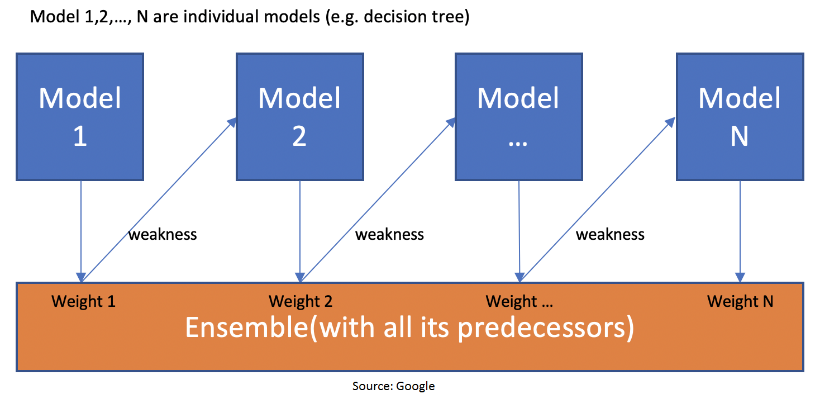
\includegraphics[scale=0.5]{Ada_boost.png}}
\caption{ AdaBoosting makes n number of decision trees during the training period of data. As the first decision tree/model is made, the record which is incorrectly classified during the first model is given more priority. Only these records are sent as input for the second model. The process will go on until we specify a number of base learners we want to create.}
\label{fig 4}
\end{figure}
\section{Non-Frontal face detection methods}
One of the most challenging tasks in building a face recognition system is how to represent and extract good quality features from face images. The most suitable method to find facial features using Viola-Jones algorithm and then use LBP (Local Binary Patterns) to find and detect the non-frontal faces.[3]
in order to save computational time, we have to limit identification to four angles i.e. left profile $(-90^{\circ},-60^{\circ})$ , left half-profile$(-60^{\circ},-30^{\circ})$,right half-profile$(30^{\circ},60^{\circ})$ \& right profile$(60^{\circ},90^{\circ})$. Furthermore , we can decrease the dataset size by flipping the images to find the face-masks; This way, we reduce training and data size by 50%.
\begin{figure}[h!]
\centerline{
\includegraphics[scale=0.3]{face.jpg}}
\caption{Different angles used for non frontal face detection}
\label{fig 5}
\end{figure}
\subsection*{Local Binary Patterns}
Local Binary Pattern (LBP) is a simple yet very efficient texture operator which labels the pixels of an image by thresholding the neighbourhood of each pixel and considers the result as a binary number. Due to its discriminative power and computational simplicity, LBP texture operator has become a popular approach in various applications. It can be seen as a unifying approach to the traditionally divergent statistical and structural models of texture analysis.[5] Perhaps the most important property of the LBP operator in real-world applications is its robustness to monotonic gray-scale changes caused, for example, by illumination variations. Another important property is its computational simplicity, which makes it possible to analyse images in challenging real-time settings.[6]\\
\begin{figure}[h!]
\centerline{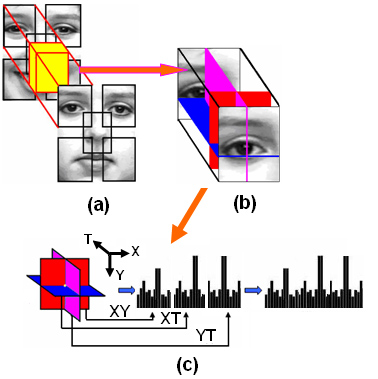
\includegraphics[scale=0.55]{LBP_Main_Facial.jpg}}
\caption{Description of facial expressions with local binary patterns}
\label{fig 6}
\end{figure}
\\ 
In the LBP approach for texture classification, the occurrences of the LBP codes in an image are collected into a histogram. The classification is then performed by computing simple histogram similarities. However, considering a similar approach for facial image representation results in a loss of spatial information and therefore one should codify the texture information while retaining also their locations. One way to achieve this goal is to use the LBP texture descriptors to build several local descriptions of the face and combine them into a global description. Such local descriptions have been gaining interest lately which is understandable given the limitations of the holistic representations. These local feature based methods are more robust against variations in pose or illumination than holistic methods.[4]\\
The basic methodology for LBP based face description proposed by Ahonen et al. (2006) is as follows: The facial image is divided into local regions and LBP texture descriptors are extracted from each region independently. The descriptors are then concatenated to form a global description of the face, as shown in Fig. 7.
\begin{figure}[h!]
\centerline{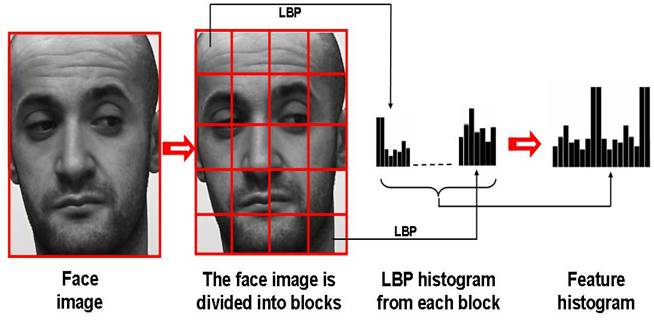
\includegraphics[scale=0.7]{LBP-face.jpg}}
\caption{Face description with local binary patterns.}
\label{fig 7}
\end{figure}
This histogram effectively has a description of the face on three different levels of locality: the LBP labels for the histogram contain information about the patterns on a pixel-level, the labels are summed over a small region to produce information on a regional level and the regional histograms are concatenated to build a global description of the face.
\\
It should be noted that when using the histogram based methods the regions do not need to be rectangular. Neither do they need to be of the same size or shape, and they do not necessarily have to cover the whole image. It is also possible to have partially overlapping regions.
\section{Deep Neural Networks}
A deep neural network (DNN) is an artificial neural network (ANN) with multiple layers between the input and output layers. There are different types of neural networks but they always consist of the same components: neurons, synapses, weights, biases, and functions. These components functioning similar to the human brains and can be trained like any other ML algorithm.\\
For example, a DNN that is trained to recognize dog breeds will go over the given image and calculate the probability that the dog in the image is a certain breed. The user can review the results and select which probabilities the network should display (above a certain threshold, etc.) and return the proposed label. Each mathematical manipulation as such is considered a layer, and complex DNN have many layers, hence the name "deep" networks.\\
DNNs can model complex non-linear relationships. DNN architectures generate compositional models where the object is expressed as a layered composition of primitives. The extra layers enable composition of features from lower layers, potentially modelling complex data with fewer units than a similarly performing shallow network. For instance, it was proved that sparse multivariate polynomials are exponentially easier to approximate with DNNs than with shallow networks.Convolutional deep neural networks (CNNs) are used in computer vision.
\subsection{Convolutional Neural Networks}
In deep learning, a convolutional neural network (CNN, or ConvNet) is a class of deep neural network, most commonly applied to analyze visual imagery. They are also known as shift invariant or space invariant artificial neural networks (SIANN), based on the shared-weight architecture of the convolution kernels or filters that slide along input features and provide translation equivariant responses known as feature maps. Counter-intuitively, most convolutional neural networks are only equivariant, as opposed to invariant, to translation. They have applications in image and video recognition, recommender systems, image classification, image segmentation, medical image analysis, natural language processing, brain-computer interfaces, and financial time series.
\\
CNNs are regularized versions of multilayer perceptrons. Multilayer perceptrons usually mean fully connected networks, that is, each neuron in one layer is connected to all neurons in the next layer. The "full connectivity" of these networks make them prone to overfitting data. Typical ways of regularization, or preventing overfitting, include: penalizing parameters during training (such as weight decay) or trimming connectivity (skipped connections, dropout, etc.) CNNs take a different approach towards regularization: they take advantage of the hierarchical pattern in data and assemble patterns of increasing complexity using smaller and simpler patterns embossed in their filters. Therefore, on a scale of connectivity and complexity, CNNs are on the lower extreme.\\
A CNN architecture is formed by a stack of distinct layers that transform the input volume into an output volume (e.g. holding the class scores) through a differentiable function. A few distinct types of layers are commonly used. These are further discussed below.
\subsubsection{Convolutional layer}
The convolutional layer is the core building block of a CNN. The layer's parameters consist of a set of learnable filters (or kernels), which have a small receptive field, but extend through the full depth of the input volume. During the forward pass, each filter is convolved across the width and height of the input volume, computing the dot product between the filter entries and the input, producing a 2-dimensional activation map of that filter. As a result, the network learns filters that activate when it detects some specific type of feature at some spatial position in the input.[8]\\ 
\begin{figure}[h]
\centerline{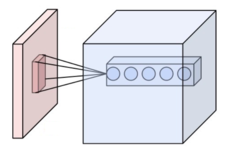
\includegraphics[scale=0.7]{Conv_layer.png}}
\caption{Neurons of a convolutional layer (blue), connected to their receptive field (red).}
\label{fig 8}
\end{figure}
Stacking the activation maps for all filters along the depth dimension forms the full output volume of the convolution layer. Every entry in the output volume can thus also be interpreted as an output of a neuron that looks at a small region in the input and shares parameters with neurons in the same activation map.[9]
\subsubsection{Local connectivity}
When dealing with high-dimensional inputs such as images, it is impractical to connect neurons to all neurons in the previous volume because such a network architecture does not take the spatial structure of the data into account. Convolutional networks exploit spatially local correlation by enforcing a sparse local connectivity pattern between neurons of adjacent layers: each neuron is connected to only a small region of the input volume.\\
The extent of this connectivity is a hyperparameter called the receptive field of the neuron. The connections are local in space (along width and height), but always extend along the entire depth of the input volume. Such an architecture ensures that the learnt filters produce the strongest response to a spatially local input pattern.[11]
\begin{figure}[h]
\centerline{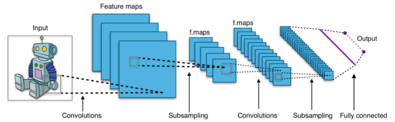
\includegraphics[scale=1]{395px-Typical_cnn.png}}
\caption{Typical CNN architecture.}
\label{fig 9}
\end{figure}
\subsubsection{Pooling layer}
Another important concept of CNNs is pooling, which is a form of non-linear down-sampling. There are several non-linear functions to implement pooling, where max pooling is the most common. It partitions the input image into a set of rectangles and, for each such sub-region, outputs the maximum.[7]\\
Intuitively, the exact location of a feature is less important than its rough location relative to other features. This is the idea behind the use of pooling in convolutional neural networks. The pooling layer serves to progressively reduce the spatial size of the representation, to reduce the number of parameters, memory footprint and amount of computation in the network, and hence to also control overfitting. This is known as down-sampling It is common to periodically insert a pooling layer between successive convolutional layers (each one typically followed by an activation function, such as a ReLU layer) in a CNN architecture. While pooling layers contribute to local translation invariance, they do not provide global translation invariance in a CNN, unless a form of global pooling is used. The pooling layer commonly operates independently on every depth, or slice, of the input and resizes it spatially. A very common form of max pooling is a layer with filters of size 2$\times$2, applied with a stride of 2, which subsamples every depth slice in the input by 2 along both width and height, discarding 75\% of the activations:
\[\displaystyle f_{X,Y}(S)=\max _{a,b=0}^{1}S_{2X+a,2Y+b}.\]
In this case, every max operation is over 4 numbers. The depth dimension remains unchanged (this is true for other forms of pooling as well)[9].\\
In addition to max pooling, pooling units can use other functions, such as average pooling or $l$2-norm pooling. Average pooling was often used historically but has recently fallen out of favor compared to max pooling, which generally performs better in practice.\\
Due to the effects of fast spatial reduction of the size of the representation, there is a recent trend towards using smaller filters or discarding pooling layers altogether.
\begin{figure}[h]
\centerline{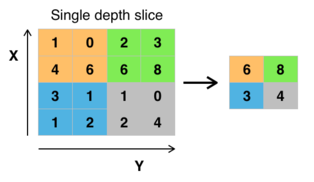
\includegraphics[scale=1]{314px-Max_pooling.png}}
\caption{Max pooling with 2$\times$2 filter and stride = 2.}
\label{fig 10}
\end{figure}
\subsection{ReLU layer}
ReLU is the abbreviation of rectified linear unit, which applies the non-saturating activation function $\textstyle f(x)=\max(0,x)$ It effectively removes negative values from an activation map by setting them to zero. It introduces non-linearities to the decision function and in the overall network without affecting the receptive fields of the convolution layers.[11]

Other functions can also be used to increase non-linearity, for example the saturating hyperbolic tangent $\displaystyle f(x)=\tanh(x)$, $\displaystyle f(x)=|\tanh(x)|$, and the sigmoid function $\textstyle \sigma (x)=(1+e^{-x})^{-1}$. ReLU is often preferred to other functions because it trains the neural network several times faster without a significant penalty to generalization accuracy.
\subsection{Fully Connected Layer}
After several convolutional and max pooling layers, the final classification is done via fully connected layers. Neurons in a fully connected layer have connections to all activations in the previous layer, as seen in regular (non-convolutional) artificial neural networks. Their activations can thus be computed as an affine transformation, with matrix multiplication followed by a bias offset (vector addition of a learned or fixed bias term).
\subsection{Loss Layer}
The "loss layer", or "loss function", specifies how training penalizes the deviation between the predicted output of the network, and the true data labels (during supervised learning). Various loss functions can be used, depending on the specific task.
\\
The Softmax loss function is used for predicting a single class of K mutually exclusive classes. Sigmoid cross-entropy loss is used for predicting K independent probability values in $\displaystyle [0,1]$. Euclidean loss is used for regressing to real-valued labels $\displaystyle (-\infty ,\infty )$. 
\section{Face Mask Detection}
Due to the Coronavirus pandemic, Face Masks have become an integral part
of our society, hence numerous implementations of detecting face mask have
come forward which are based on Convolutional Neural Networks. [12] proposed a two stage detection scheme, the first being face detection, and the next
being face mask classifier. [13] proposed a hybrid deep transfer learning model
with two components, the first for feature extraction using ResNet50 and other for classification using SVM, and other ensemble algorithms. Their Support Vector Machine (SVM) classifier achieved testing accuracy of 99.64\%. RetinaMask [14] achieved state-of-the-art result on public face mask dataset (2.3\% and 1.5\% higher precision than baseline result on face and mask detection) using one-stage detector which consisted of feature pyramid network to fuse high level semantic information with multiple feature maps. [15] presented a model with pre-trained weights of VGG-16 architecture for feature extraction and then a fully connected neural network (FCNN) to segment out faces present in an image, and detect face
masks on them. The model showed great result in recognizing non-frontal faces.
[16] proposed a model using YOLO-v2 with ResNet-50 which achieves higher
average precision by using mean Intersection over Union (IoU). [17] proposed
a model based on transfer learning with InceptionV3, It outperformed recently
proposed models by achieving testing accuracy of 100\% on Simulated Masked
Face Dataset (SMFD). [18] discussed the challenge of implementing object detection on edge devices, the paper compared various popular object detection
algorithms like YOLO-v3, YOLO-v3tiny, Faster R-CNN, etc. to determine the
most efficient algorithm for real time detection of face masks.
\subsection{Quantization}
Leveraging quantization techniques is necessary for implementing CNNs on
resource-constrained devices. [19] introduced 4-bit training quantization on both
activation and weights, achieving accuracies, a few percent less than state-of the-art baselines across CNNs. [20] proposed a method which quantizes layer
parameters that improve accuracy over existing post-training quantization techniques. [21] proposed an outlier channel splitting (OCS) based method to improve quantization performance without retraining. [22] discussed low bit quantization of neural networks by optimization of constrained Mean Squared Error(MSE) problems for performing hardware-aware quantization. [23] proposed a quantization scheme along with a co-designed training procedure. The paper concluded that inference using integer-only arithmetic performs better than
floating-point arithmetic on typical ARM CPUs. [24] proposed Differentiable Soft
Quantization (DSQ) to bridge the gap between the full-precision and low-bit
networks. The hybrid compression model in [21] uses four major modules, Approximation, Quantization, Pruning, and Coding, which provides 20-30$\times$  compression rate with negligible loss in accuracy. The research by [25], [26], and [27]
proposed mixed-precision quantization techniques, where more sensitive layers
are at higher precision.


\section{ Power Demanding Facemask Detection models}
This section discusses two models of face mask detection whuch use the least computational power.
\subsection{Face Mask Detection Using Single Shot Dultibox Detector \& MobilenetV2}
Face mask detection had seen significant progress in the domains of Image processing and Computer vision, since the rise of the Covid-19 pandemic. Many face detection models have been created using several algorithms and techniques. The proposed approach in [28] uses deep learning, TensorFlow, Keras, and OpenCV to detect face masks. This model can be used for safety purposes since it is very resource efficient to deploy. The SSDMNV2 approach uses Single Shot Multibox Detector as a face detector and MobilenetV2 architecture as a framework for the classifier, which is very lightweight and can even be used in embedded devices (like NVIDIA Jetson Nano, Raspberry pi) to perform real-time mask detection. The technique deployed in this model gives us an accuracy score of 0.9264 and an F1 score of 0.93. The flow diagram of the model is shown in fig 11.
\begin{figure}[h]
\centerline{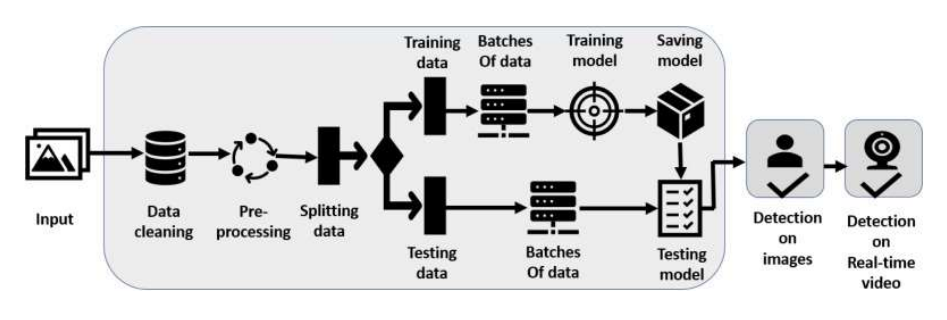
\includegraphics[scale=.6]{ssdmnv2.png}}
\caption{Flow diagram of the ssdmnv2 model}
\label{fig 11}
\end{figure}
The SSDMNV2 model was also compared with different pre-existing models like LeNet-5, AlexNet, VGG-16, and ResNet-50 by training them on the same dataset, and the proposed model outperforms the other models in terms of accuracy, F1 score and FPS parameter. As a result SSDMNV2 model is easy to deploy on embedded devices which is not possible with heavy models and to do real-time detection using these models that requires good computational power and which is the sole purpose of the research.
\subsection{Learning based Safe Social Distancing and Face Mask Detection in Public Areas for COVID-19 Safety Guidelines Adherence}
\begin{figure}[h]
\centerline{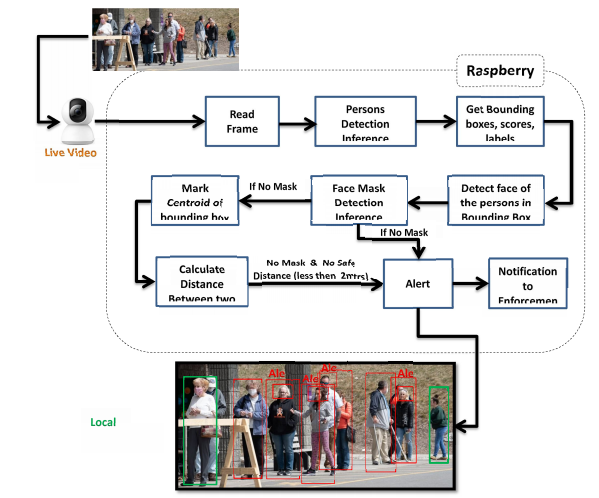
\includegraphics[scale=.8]{PUBLIC.png}}
\caption{flow diagram of the proposed system}
\label{fig 11}
\end{figure}
A novel coronavirus has resulted in person-to-person transmission but as far as we know, the transmission of the novel coronavirus causing coronavirus disease 2019 (COVID-19) can also be from an asymptomatic carrier with no covid symptoms. Till now there is no report about any clinically approved antiviral medicine or vaccines that are effective against 
$COVID-19$. It has spread rapidly across the world, bringing massive health, economic, environmental and social challenges to the entire human population. At the moment, WHO recommends that people should wear face masks to avoid the risk of virus transmission and also recommends that a social distance of at least 2 mtrs  be maintained between individuals to prevent person to person spread of disease. Furthermore, many public service providers require customers to use the service only if they wear masks and follow safe social distancing. Therefore, face mask detection and safe social distance monitoring has become a crucial computer vision task to help the global society. [29] describes approach to prevent the spread of the virus by monitoring in real time if person is following safe social distancing and wearing face masks in public places. This model adopts a combination of lightweight neural network MobileNetV2 and Single Shot Detector(SSD) with transfer learning technique to achieve the balance of resource limitations and recognition accuracy so that it can be used on real-time video surveillance to monitor public places to detect if persons wearing face mask and maintaining safe social distancing. This solution uses neural networking models to analyze Real-Time Streaming Protocol (RTSP) video streams using OpenCV and MobileNet V2. 
We mix the approach of modern-day deep learning and classic projective geometry techniques which not only helps to meet the real-time requirements, but also keeps high prediction accuracy. If the person detected as not following the covid-19 safety 
guidelines, violation alerts will be send to the control center at state police headquarters for taking further action. It allows 
automating the solution and enforces the wearing of the mask and follows the guidelines of social distancing. This model was created to run on raspberry pi4 and the accuracy obtained was between 85\% and 95\%.
\section*{Conclusion}
Face mask detection is an effective method that can be used to prevent the spread of $COVID-19$. This can be done in three ways, i.e. using just machine algorithms or using Deep Neural Networks or as a hybrid i.e. a mix of machine learning and DNN.\\ It was found that the hybrid and DNN approaches have high accuracies while the machine learning approach has a comparably lower accuracy for face mask detection. 
\section*{References}
\begin{enumerate}
\item Viola and Jones, "Rapid object detection using a boosted cascade of simple features", Computer Vision and Pattern Recognition, 2001
\item Lienhart, R. and Maydt, J., "An extended set of Haar-like features for rapid object detection", ICIP02, pp. I: 900–903, 2002
\item Ahonen, T., Hadid, A. and Pietikäinen, M. (2006), Face Description with Local Binary Patterns: Application to Face Recognition. IEEE Trans. Pattern Analysis and Machine Intelligence 28(12):2037-2041.
\item  Y. Amit, D. Geman, and K. Wilder. Joint induction of shape features and tree
classifiers, 1997.
\item Heikkilä, M., Pietikäinen, M. and Schmid, C. (2009), Description of Interest Regions with Local Binary Patterns. Pattern Recognition 42(3):425-436.
\item Ojala, T., Pietikäinen, M. and Harwood, D. (1996), A Comparative Study of Texture Measures with Classification Based on Feature Distributions. Pattern Recognition 19(3):51-59.
\item Scherer, Dominik; Müller, Andreas C.; Behnke, Sven (2010). "Evaluation of Pooling Operations in Convolutional Architectures for Object Recognition" (PDF). Artificial Neural Networks (ICANN), 20th International Conference on. Thessaloniki, Greece: Springer. pp. 92–101.
\item Mouton, Coenraad; Myburgh, Johannes C.; Davel, Marelie H. (2020). Gerber, Aurona (ed.). "Stride and Translation Invariance in CNNs". Artificial Intelligence Research. Communications in Computer and Information Science. Cham: Springer International Publishing. 1342: 267–281. arXiv:2103.10097. doi:10.1007/978-3-030-66151-$9_17$. ISBN 978-3-030-66151-9. S2CID 232269854
\item "Convolutional Neural Networks (LeNet) – DeepLearning 0.1 documentation". DeepLearning 0.1. LISA Lab. Retrieved 31 August 2013.
\item Venkatesan, Ragav; Li, Baoxin (2017-10-23). Convolutional Neural Networks in Visual Computing: A Concise Guide. CRC Press. ISBN 978-1-351-65032-8.
\item Ciresan, Dan; Meier, Ueli; Schmidhuber, Jürgen (June 2012). Multi-column deep neural networks for image classification. 2012 IEEE Conference on Computer Vision and Pattern Recognition. New York, NY: Institute of Electrical and Electronics Engineers (IEEE). pp. 3642–3649. arXiv:1202.2745
\item Chavda, A., Dsouza, J., Badgujar, S., Damani, A.: Multi-Stage CNN Architecture
for Face Mask Detection. arXiv e-prints arXiv:2009.07627 (2020)
\item Loey, M., Manogaran, G., Taha, M., Khalifa, N.: A hybrid deep transfer learning model with machine learning methods for face mask detection in the era of
the covid-19 pandemic. Measurement: Journal of the International Measurement
Confederation 167 (2021). DOI 10.1016/j.measurement.2020.108288
\item Jiang, M., Fan, X., Yan, H.: RetinaMask: A Face Mask detector. arXiv e-prints
arXiv:2005.03950 (2020)
\item Meenpal, T., Balakrishnan, A., Verma, A.: Facial mask detection using semantic
segmentation. In: 2019 4th International Conference on Computing, Communications and Security (ICCCS), pp. 1–5 (2019). DOI 10.1109/CCCS.2019.8888092
\item Loey, M., Manogaran, G., Taha, M.H.N., Khalifa, N.E.M.: Fighting against covid19: A novel deep learning model based on yolo-v2 with resnet-50 for medical face
mask detection. Sustainable Cities and Society p. 102600 (2020). DOI https:
//doi.org/10.1016/j.scs.2020.102600. URL http://www.sciencedirect.com/science/
article/pii/S2210670720308179
\item Jignesh Chowdary, G., Singh Punn, N., Sonbhadra, S.K., Agarwal, S.: Face Mask
Detection using Transfer Learning of InceptionV3. arXiv e-prints arXiv:2009.08369
(2020)
\item Banner, R., Nahshan, Y., Soudry, D.: Post training 4-bit quantization of convolutional networks for rapid-deployment. In: H. Wallach, H. Larochelle,
A. Beygelzimer, F. d'Alch´e-Buc, E. Fox, R. Garnett (eds.) Advances in
Neural Information Processing Systems, vol. 32, pp. 7950–7958. Curran Associates, Inc. (2019). URL https://proceedings.neurips.cc/paper/2019/file/
c0a62e133894cdce435bcb4a5df1db2d-Paper.pdf
\item Nahshan, Y., Chmiel, B., Baskin, C., Zheltonozhskii, E., Banner, R., Bronstein,
A.M., Mendelson, A.: Loss Aware Post-training Quantization. arXiv e-prints
arXiv:1911.07190 (2019)
\item Zhao, R., Hu, Y., Dotzel, J., De Sa, C., Zhang, Z.: Improving neural network
quantization without retraining using outlier channel splitting. In: K. Chaudhuri,
R. Salakhutdinov (eds.) Proceedings of the 36th International Conference on Machine Learning, Proceedings of Machine Learning Research, vol. 97, pp. 7543–7552.
PMLR, Long Beach, California, USA (2019). URL http://proceedings.mlr.press/
v97/zhao19c.html
\item Choukroun, Y., Kravchik, E., Yang, F., Kisilev, P.: Low-bit quantization of neural
networks for efficient inference. In: 2019 IEEE/CVF International Conference
on Computer Vision Workshop (ICCVW), pp. 3009–3018 (2019). DOI 10.1109/
ICCVW.2019.00363
\item Jacob, B., Kligys, S., Chen, B., Zhu, M., Tang, M., Howard, A., Adam, H.,
Kalenichenko, D.: Quantization and training of neural networks for efficient integerarithmetic-only inference. In: Proceedings of the IEEE Conference on Computer
Vision and Pattern Recognition (CVPR) (2018)
\item Gong, R., Liu, X., Jiang, S., Li, T., Hu, P., Lin, J., Yu, F., Yan, J.: Differentiable
soft quantization: Bridging full-precision and low-bit neural networks. In: Proceedings of the IEEE/CVF International Conference on Computer Vision (ICCV)
(2019)
\item Ge, S., Luo, Z., Zhao, S., Jin, X., Zhang, X.: Compressing deep neural networks for
efficient visual inference. In: 2017 IEEE International Conference on Multimedia
and Expo (ICME), pp. 667–672 (2017). DOI 10.1109/ICME.2017.8019465
\item Dong, Z., Yao, Z., Gholami, A., Mahoney, M.W., Keutzer, K.: Hawq: Hessian
aware quantization of neural networks with mixed-precision. In: Proceedings of
the IEEE/CVF International Conference on Computer Vision (ICCV) (2019)
\item Dong, Z., Yao, Z., Cai, Y., Arfeen, D., Gholami, A., Mahoney, M.W., Keutzer,
K.: Hawq-v2: Hessian aware trace-weighted quantization of neural networks. In:
Advances in Neural Information Processing Systems 33 pre-proceedings (NeurIPS
2020) (2019)
\item Yao, Z., Dong, Z., Zheng, Z., Gholami, A., Yu, J., Tan, E., Wang, L., Huang,
Q., Wang, Y., Mahoney, M.W., Keutzer, K.: HAWQV3: Dyadic Neural Network
Quantization. arXiv e-prints arXiv:2011.10680 (2020)
\item Preeti Nagrath, Rachna Jain, Agam Madan, Rohan Arora, Piyush Kataria, Jude Hemanth,
SSDMNV2: A real time DNN-based face mask detection system using single shot multibox detector and MobileNetV2,Sustainable Cities and Society,Volume 66,2021,102692,ISSN 2210-6707, https://doi.org/10.1016/j.scs.2020.102692.
\item Shashi Yadav.Deep Learning based Safe Social Distancing and Face Mask Detection in Public Areas for COVID-19 Safety Guidelines AdherenceInternational Journal for Research in Applied Science \& Engineering Technology (IJRASET),Volume 8 Issue VII July 2020, ISSN: 2321-9653
\end{enumerate}
\end{document}